%
% File acl2018.tex
%
%% Based on the style files for ACL-2017, with some changes, which were, in turn,
%% Based on the style files for ACL-2015, with some improvements
%%  taken from the NAACL-2016 style
%% Based on the style files for ACL-2014, which were, in turn,
%% based on ACL-2013, ACL-2012, ACL-2011, ACL-2010, ACL-IJCNLP-2009,
%% EACL-2009, IJCNLP-2008...
%% Based on the style files for EACL 2006 by 
%%e.agirre@ehu.es or Sergi.Balari@uab.es
%% and that of ACL 08 by Joakim Nivre and Noah Smith

\documentclass[11pt,a4paper]{article}
\usepackage[hyperref]{acl2018}
\usepackage{times}
\usepackage{latexsym}
\usepackage{url}
\usepackage{multirow}
\usepackage{amssymb}
\usepackage{amsmath}
\usepackage{hyperref}
\usepackage{algorithm}
\usepackage{algpseudocode}
\usepackage{graphicx}

%\aclfinalcopy % Uncomment this line for the final submission
\def\aclpaperid{1355} %  Enter the acl Paper ID here

%\setlength\titlebox{5cm}
% You can expand the titlebox if you need extra space
% to show all the authors. Please do not make the titlebox
% smaller than 5cm (the original size); we will check this
% in the camera-ready version and ask you to change it back.

\newcommand\BibTeX{B{\sc ib}\TeX}


\title{Toward Featureless Event Coreference Resolution via Conjoined Convolutional Neural Networks}


\author{Chris Tanner \textnormal{and} Eugene Charniak\\
Brown Linguistic Laboratory of Information Processing \\
  Brown University \\
  Providence, RI  02912 \\
  {\tt \{christanner,ec\}@cs.brown.edu} \\}

\date{}

\begin{document}
\maketitle
\begin{abstract}
% motivation / others' weaknesses
Coreference resolution systems for entities and/or events almost always make use of many linguistic, parsing-based features.  In contrast, (1) we introduce a new state-of-the-art event coreference resolution system which uses only lemmatization and its corresponding precomputed word/character embeddings, and we exhaustively illustrate the performance of other commonly-used features.  (2) The crux of our system is that it first makes pairwise event-coreference predictions by using a Conjoined Convolutional Neural Network.  Last, (3) we cluster event mentions with a novel neural approach which performs merges in an easy-first, cluster-holistic manner, allowing our system to be less susceptible to errors that are made exclusively from min-pairwise decisions.  When performed on a common test set of the ECB+ corpus, our system achieves CoNLL F1 scores of 67.2 and 59.3 for within-document and cross-document tasks, respectively.
\end{abstract}

%%%%%%%%%%%%%%%%%%%%%%%%%%%%%%%%%%%%%%%%%%%%%%%%%
%%%%%%%%%%%%%%                     1.  INTRODUCTION                   %%%%%%%%%%%%%%%
%%%%%%%%%%%%%%%%%%%%%%%%%%%%%%%%%%%%%%%%%%%%%%%%%

\section{Introduction}
% problem definition/statement
Coreference resolution is the task of identifying -- within a single text or across multiple documents -- which \textit{mentions} refer to the same underlying discourse \textit{entity} or \textit{event}.  A \textit{mention} is a particular instance of word(s) in a document (e.g., \textit{she} or \textit{announced}).  Ultimately, coreference resolution is a clustering task, whereby we wish to group all like-mentions together, as shown in Figure \ref{fig:corpus}.  Successfully doing so can be useful for other core NLP tasks, such as information extraction \cite{Humphreys:1997}, topic detection \cite{Allan:1998}, and summarization \cite{Daniel:2003}.

\begin{figure}[ht]
\centering
	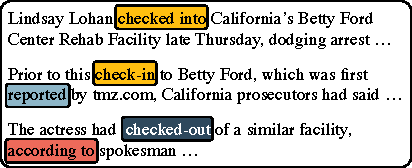
\includegraphics[width=0.45\textwidth]{corpus}
	\caption{Sample of the ECB+ corpus, depicting gold coref mentions as having shared box colors.}
	\label{fig:corpus}
\end{figure}

% problem definition
Coreference systems aim to find a globally-optimal fit of mentions to clusters, whereby every mention $m$ in the corpus is assigned to exactly one cluster $C$, such that every ${m_i,m_j} \in C$ are co-referent with each other.  If a given $m_i$ is not anaphoric with any other $m_j$, then it should belong to its own $C$ with a membership of one.  Finding a globally-optimal assignment of clusters is NP-Hard and thus computationally intractable.  In attempt to avoid this, systems typically perform pairwise-mention predictions, then use those predictions to build clusters. The specific modelling strategies for such approximately fall into two categories: (1) mention-ranking / mention-pairs; and (2) entity-level / event-level.

\textbf{Mention-ranking} models define a scoring function $f(m_i,m_j)$ which operates on a mention $m_j$ and possible antecedent $m_i$, where $m_i$ occurs earlier in the document and could be null (represented by $\epsilon$ and denoting that $m_j$ is non-anaphoric); e.g., Wiseman, et. al.'s \shortcite{DBLP:journals/corr/WisemanRS16}.

\textbf{Mention-pair} models score all pairs ($m_i,m_j)$, in contrast to mention-ranking models which aim to find the ideal $m_i$ antecedent for every $m_j$.  Because these models base their predictions on the information from just two mentions at a time, they are by definition less expressive than entity/event-level models.  Yet, their inference can be relatively simple and effective, allowing them to be fast and scalable.  Consequently, they have often been the approach used by many state-of-the-art systems \cite{Soon:2001:MLA:972597.972602,DBLP:conf/emnlp/DurrettK13}.

\textbf{Entity/Event-level} models differ in that they focus on building a global representation of each underlying entity or event, the basis of which determines each mention's membership -- as opposed to operating on a mention-level basis \cite{DBLP:journals/corr/WisemanRS16,clark2016improving}.

In this work, we use a novel mention-pair model that is designed to discriminate between pairs of input features: Siamese Convolutional Neural Networks.  We feel awkward using the term ``siamese,'' so we will henceforth refer to our model as our newly-coined term, Conjoined Convolutional Neural Networks (or CCNN).  Further, we aim to replace a common weakness of mention-pair models with an approach resembling the main strength of entity/event-level models. Specifically, we aim to combine all linked mention pairs into a cluster via a neural, easy-first clustering approach which factors in a small, but effective, notion of the entire cluster at large.

Additionally, coreference research systems typically use a plethora of relatively expensive parsing-based features, including dependency parse information, lemmatization, WordNet hypernyms/synonyms, FrameNet semantic roles, etc.  Although some research papers list their system's learned feature weights \cite{journals/tacl/YangCF15}, there has been a striking lack of work which takes the minimalist approach and illustrates the effects of using few features.  We aim to address this by starting with a basic lemma-embedding feature and then evaluate on our dev set the effectiveness of adding other commonly used features.

In summary, we are interested in within-document and cross-document \textit{event} coreference, which has received drastically less attention than \textit{entity} coreference. We introduce a novel mention-pair approach, using a Conjoined Convolutional Neural Network and unusually few features.  We contribute detailed results of other commonly used features.  And last, we combine our predicted mention pairs into clusters via a simple neural approach which represents each cluster as a whole, yielding state-of-the-art results on the ECB+ corpus.

%%%%%%%%%%%%%%%%%%%%%%%%%%%%%%%%%%%%%%%%%%%%%%%%%
%%%%%%%%%%%%%%                 2.   RELATED        WORK               %%%%%%%%%%%%%%%
%%%%%%%%%%%%%%%%%%%%%%%%%%%%%%%%%%%%%%%%%%%%%%%%%

\section{Related Work}
% initial start
The seminal research on event coreference can be traced back to the DARPA-initiated MUC conferences, whereby the focus was on limited scenarios involving terrorist attacks, plane crashes, management succession, resignation, etc. \cite{Humphreys:1997,Bagga:1999:CEC:1608810.1608812}.

In the present day, Deep Learning is revolutionizing NLP; however, there has been few successful applications of deep learning to coreference, almost all of which have been for \textit{entity} coreference.  We attribute this dearth to the fact that coreference resolution is inherently a clustering task, which tends to be a non-obvious modality for deep learning.  Since our model (1) uses deep learning and (2) operates on the ECB+ corpus, we organize the related research accordingly.

\subsection{Deep Learning Approaches}
To the best of our knowledge, there are only five publications which apply deep learning to coreference resolution, four of which focus on entity coreference.

Sam Wiseman, et. al. \shortcite{DBLP:conf/acl/WisemanRSW15,DBLP:conf/naacl/WisemanRS16} trained a mention-ranking model with a heuristic loss function that assigns different costs based on the types of errors made, and their latter work used mention-ranking predictions towards an entity-level model.
Clark and Manning \shortcite{clark2016improving,DBLP:journals/corr/ClarkM16a} also built both a mention-ranking model and an entity-level model, the former of which was novel in using reinforcement learning to find the optimal loss values for the same four distinct error types defined in Wiseman's, et. al. \shortcite{DBLP:conf/acl/WisemanRSW15} work.

\subsection{Systems using ECB+ Corpus}
% most related
For our research, we make use of the ECB+ corpus \cite{ECB+}, which we further describe in Section \ref{sec:corpus}.  This rich corpus provides annotations for both entities and events, yet most research chooses to focus on using \textit{either} events \textit{or} entities, not both.  To the best of our knowledge, there are only two papers which focus on the event mentions of ECB+: The Hierarchical Distance-dependent Chinese Restaurant Process (HDDCRP) model by Yang, et. al. \shortcite{journals/tacl/YangCF15} and Choubey's and Huang's Iteratively-Unfolding approach \shortcite{Choubey2017EventCR}.

\subsubsection{HDDCRP Model}
\label{sec:HDDCRP}
% HDDCRP
Yang, et. al's HDDCRP model \shortcite{journals/tacl/YangCF15} uses a clever mention-pair approach, whereby they first use logistic regression to train parameters $\theta$ for the similarity function in Equation \ref{eq:hddcrp}.  
\begin{equation}
\label{eq:hddcrp}
f_{\theta}(x_i,x_j) \propto \textnormal{exp\{} \theta^T\psi(m_i,m_j)\textnormal{\}}
\end{equation}
Then, in a Chinese-restaurant-process fashion, they probabilistically link together mentions based purely on the scores provided by this similarity function.  That is, the value of $f(m_i,m_j)$ is directly correlated with the probability of $(m_i,m_j)$ being chosen as a linked pair.  Then, identical to Bengtson's and Roth's work \shortcite{Bengtson:2008:UVF:1613715.1613756}, the HDDCRP model forms clusters by tracing through all linked pairs. All mentions that are reachable by a continuous path become assigned the same cluster.  This hinges on the transitive property of coreference.  For example, if ${(m_1,m_3),(m_3,m_5)}$ and $(m_5,m_6)$ are each individually linked via the scoring function, then a cluster $C_i$ is formed, where $C_i = \{m_1,m_3,m_5,m_6\}$, even though $(m_1,m_5)$ or $(m_3,m_6)$ may have had very low similarity scores. We aim to improve this shortcoming, as detailed in Section \ref{sec:clustering}.

\subsubsection{Neural Iteratively-Unfolding Model}
\label{sec:Choubey}
% Choubey
Recently, Choubey and Huang \shortcite{Choubey2017EventCR} introduced the first neural model for event coreference.  Their system also fits into the mention-pair paradigm, whereby mentions are predicted by a feed-forward network.  The authors asserted that when using the ECB+ corpus, within-doc coreference did not benefit from using mention context, which is an important finding.  However, similar to the weakness of the HDDCRP model, they merge clusters which contain \textit{any} mention-pair whose predicted score is below a given threshold, independent of mentions' relation to the cluster at large.

%%%%%%%%%%%%%%%%%%%%%%%%%%%%%%%%%%%%%%%%%%%%%%%%%
%%%%%%%%%%%%%%             3.  SYSTEM      OVERVIEW                %%%%%%%%%%%%%%%
%%%%%%%%%%%%%%%%%%%%%%%%%%%%%%%%%%%%%%%%%%%%%%%%%

\section{System Overview}
\subsection{Mention Identification}
\label{sec:mentionid}
Coreference systems are predicated upon having entity/event mentions identified.  In fact, this identification process is the focus of a different line of research: entity recognition and event detection.  This separation of tasks allows coreference systems to be evaluated precisely on their ability to cluster together appropriate mentions, independent from the mention detection.  Thus, it is common practice for coreference systems to either: (1) use an off-the-shelf entity recognition system, or (2) use gold mentions that are defined in the corpus.  To illustrate the effectiveness of our system, we do both, and we use the exact same set of mentions as each system we compare against:


The \textbf{HDDCRP} model does not use the gold test mentions provided by ECB+.  Instead, they used a semantic role labeller to identify and filter all test mentions.
To compare against their system, we worked with the HDDCRP source code and data to ensure we accurately use their same mentions.  Independent of clustering performance: of the 3,290 gold mentions in ECB+, their system failed to identify/use 676 of them.  Of their 3,109 predicted mentions, 495 were false positives and in fact not actual gold mentions.  Since their system uses these imperfect mentions, yet tests the coreference performance against the gold mentions, their system encounters a steep performance loss by default.  We fairly compare our system with theirs by using the same, imperfectly-predicted mentions.

The Iteratively-Unfolding system also aimed to use the same mentions as HDDCRP's.  After numerous exchanges with the author, it was clear that their set of \textit{test} mentions was similar and reasonable for research, but understandably not the same as that used by HDDCRP.  Namely, they filtered out: (1) all predicted mentions which were not in the gold set (false positives), and (2) predicted mentions which did not cluster with a mention from another document.  When we compare against this system, we followed their convention.

Lastly, to show an upper-bound of performance, we also report results having trained and tested our system using the ECB+ corpus' gold mentions.

\subsection{Reproducibility}
We provide our \href{https://drive.google.com/open?id=1iYT9kavm-r7t3YG9KRRQcQ7jtGL_KhnC}{anonymous code online}, which is written in Keras \cite{chollet2015} and is easily runnable on any of the aforementioned sets of mentions and evaluations.  Additionally, our code runs in just a few minutes on a single Titan X GPU.

\subsection{Models}
Our coreference systems are comprised of two neural models, which we describe in the next three sections.
\begin{itemize}
  \item Conjoined Convolutional Neural Network (CCNN) -- used for making mention-pair predictions.  (Section \ref{sec:CCNN})
  \item Neural Clustering (NC) -- uses CCNN's pairwise predictions to cluster mentions into events (Section \ref{sec:clustering})
\end{itemize}

\subsection{Corpus}
\label{sec:corpus}
We use the ECB+ corpus \cite{ECB+}, which is the largest available dataset with annotations for event coreference.  The corpus is comprised of 43 distinct \textit{topics}, totaling 982 documents.  We maintain the same train/dev/test splits as previous researchers, as further detailed in Section \ref{sec:coreference}.  A sample of the corpus in shown in Figure \ref{fig:corpus}, and statistics are listed in Table \ref{tab:ECB1}, where it is clear that the majority of gold mentions are one token in length (e.g, \textit{announced}).

\begin{table}
\centering
\begin{tabular}{c|c|c|c|c|}
\cline{2-5}
& Train & Dev & Test & Total \\ \cline{1-5} \hline
\multicolumn{1}{ |c| }{\# Documents} & 462 & 73 & 447 & 982   \\ %\cline{1-5}
\multicolumn{1}{ |c| }{\# Sentences} & 7,294 & 649 & 7,867 & 15,810    \\ 
%\multicolumn{1}{|c|}{\multirow{2}{*}{\pbox{2cm}{Mention\\length}}} & & & & \\ 
\multicolumn{1}{ |c| }{\# Mentions-1} & 1,938 & 386 & 2,837 & 5,161    \\ %\cline{1-5}
\multicolumn{1}{ |c| }{\# Mentions-2} & 142 & 52 & 240 & 434    \\ %\cline{1-5}
\multicolumn{1}{ |c| }{\# Mentions-3} & 18 & -- & 25 & 43    \\% \cline{1-5}
\multicolumn{1}{ |c| }{\# Mentions-4} & 6 & -- & 7 & 13   \\ \cline{1-5}
\end{tabular}
\caption{Statistics of the ECB+ Corpus, where Mentions-N represents event mentions which are N-tokens in length.}
\label{tab:ECB1}
\end{table}

%%%%%%%%%%%%%%%%%%%%%%%%%%%%%%%%%%%%%%%%%%%%%%%%%
%%%%%%%%%%%%%%                              4.   CCNN                          %%%%%%%%%%%%%%%
%%%%%%%%%%%%%%%%%%%%%%%%%%%%%%%%%%%%%%%%%%%%%%%%%

\section{Conjoined Convolutional Neural Network (CCNN)}
\label{sec:CCNN}
\subsection{Overview}
Conjoined Neural Networks (a.k.a. Siamese Networks) were first introduced by Bromly and LeCun \shortcite{SiameseNet} for the task of determining if two signatures were from the same person or not.  Specifically, Conjoined Networks are two identical neural networks, each of which accepts distinct inputs, which are joined by a single loss function over their highest-level features.  The loss function computes a similarity score (e.g., euclidean distance) for an input pair.  The networks are said to be conjoined because they share the same weights and thus work together as one network that learns how to discriminate.  The benefits of tying the weights are that it: (1) ensures that similar inputs will be mapped appropriately, otherwise, they could be mapped to hidden representations that are dissimilar from their input representations; and (2) forces the network to be symmetric. If we abstractly represent the Conjoined Network as a function, then:

$CCNN(f_i,f_j) \equiv CCNN(f_j,f_i)$

This is critical, as the CCNN's similarity function should be independent of the ordering of its input pair.

Last, Conjoined Networks have been shown to perform well in low-resource situation \cite{Koch2015SiameseNN}.  This is ideal for our task, as it is highly likely that at test time we encounter event mentions that are OOV.  We desire our model to discriminately learn the relationships of input mentions, rather than exclusively relying on the input values themselves.  Likewise, we choose to use a Convolutional Network due to (1) their power in learning sub-regions of features and the relations thereof, and (2) their recent advances in many NLP tasks \cite{DBLP:conf/emnlp/Kim14,DBLP:conf/acl/GehringAGD17,DBLP:journals/corr/YuV17}.

\subsection{Input Features}
\label{sec:features}
Since our CCNN needs each mention to be represented exclusively by its own input, we used none of the relational features\footnote{We also experimented with extending our CCNN model by adding relational features as a merged-layer at the highest neural level.} that are common in other coreference systems (e.g., SameLemma, Jaccard similarity of mentions' context, shared WordNet parents).  We used Stanford CoreNLP \cite{manning-EtAl:2014:P14-5} to extract the following features, which we thoroughly tested in different ways: % FIRST PASS DELETE (combine w/ previous paragraph)
\begin{itemize}
  \item \textbf{Part-of-Speech:} LSTM-learned POS embeddings; and 1-hot representations.
  \item \textbf{Lemmatization}: Lemmatized each token and represented it by pre-trained GloVe \cite{pennington2014glove} word embeddings.
  \item \textbf{Dependency Lemma:} we represent the dependent parent/children of each token via their aforementioned lemma embeddings.
  \item \textbf{Character Embeddings:} each token is represented as a concatenation of its character embeddings.
  \item \textbf{Word Embeddings:} pre-trained GloVe word embeddings.
\end{itemize}
We account for mentions' having varying token lengths by summing their tokens in place, thus representing each mention as a fixed-length vector.

\subsection{Architecture}
We define the full embedding for a given token $t$ as $t_{emb} = t_{f_{1}} \oplus t_{f_{2}} \oplus \ldots \oplus t_{f_{n}},$ where $\oplus$ represents vector concatenation and $t_{f_{i}}$ represents a specific input feature vector.

Naturally, we may want to convolve over the context of mention $m$, too, by including the $N$ words before and after $m$.  Thus, our input for mention $m$ is a matrix $M$, and a la Kim \shortcite{DBLP:conf/emnlp/Kim14}, we zero-pad unfilled windows.

\vspace{3mm}

Let $\textbf{M}$ represent the full matrix corresponding to mention $m$: $\textbf{M} \in \mathbb{R}^{(2N+1) \times d}$ and $\textbf{M}_{(i,j),(k:l)}$ represent the sub-matrix of $M$ from $(i,j)$ to $(k,l)$.

\vspace{3mm}

We define a kernel with dimensions $(h,w)$, where $h < (2N+1)$ and $w < d$.  This allows the kernel to operate on sub-sections of the embeddings.  The kernel has an associated weight matrix $\textbf{w} \in \mathbb{R}^{h \times w}$.  Starting at a given index $(i,j)$ within mention matrix $\textbf{M}$, a feature $c_{i}$ is defined as:
\begin{equation}
c_{i} = f(\textbf{w}^{T}\textbf{M}_{(i:i+h-1),(j:j+w-1)} + b)
\end{equation}
where $b \in \mathbb{R}$ is an added bias term.  The kernel runs over every possible sub-section of mention matrix $\textbf{M}$, yielding a feature map $\textbf{c} \in \mathbb{R}^{(2N-h) \times (d-w-1)}$

\vspace{3mm}

Since the network is comprised of two identical, conjoined halves, we sufficiently represent the architecture in Figure \ref{fig:ccnn} with just one half.  The Lambda function calculates the Euclidean distance of each half's univariate vector and emits a two-class softmax prediction regarding the likelihood of the two mentions being co-referent.  Complete parameter values such as dropout and kernel sizes are listed in our Supplemental Materials document.

\begin{figure*}[h]
\centering
	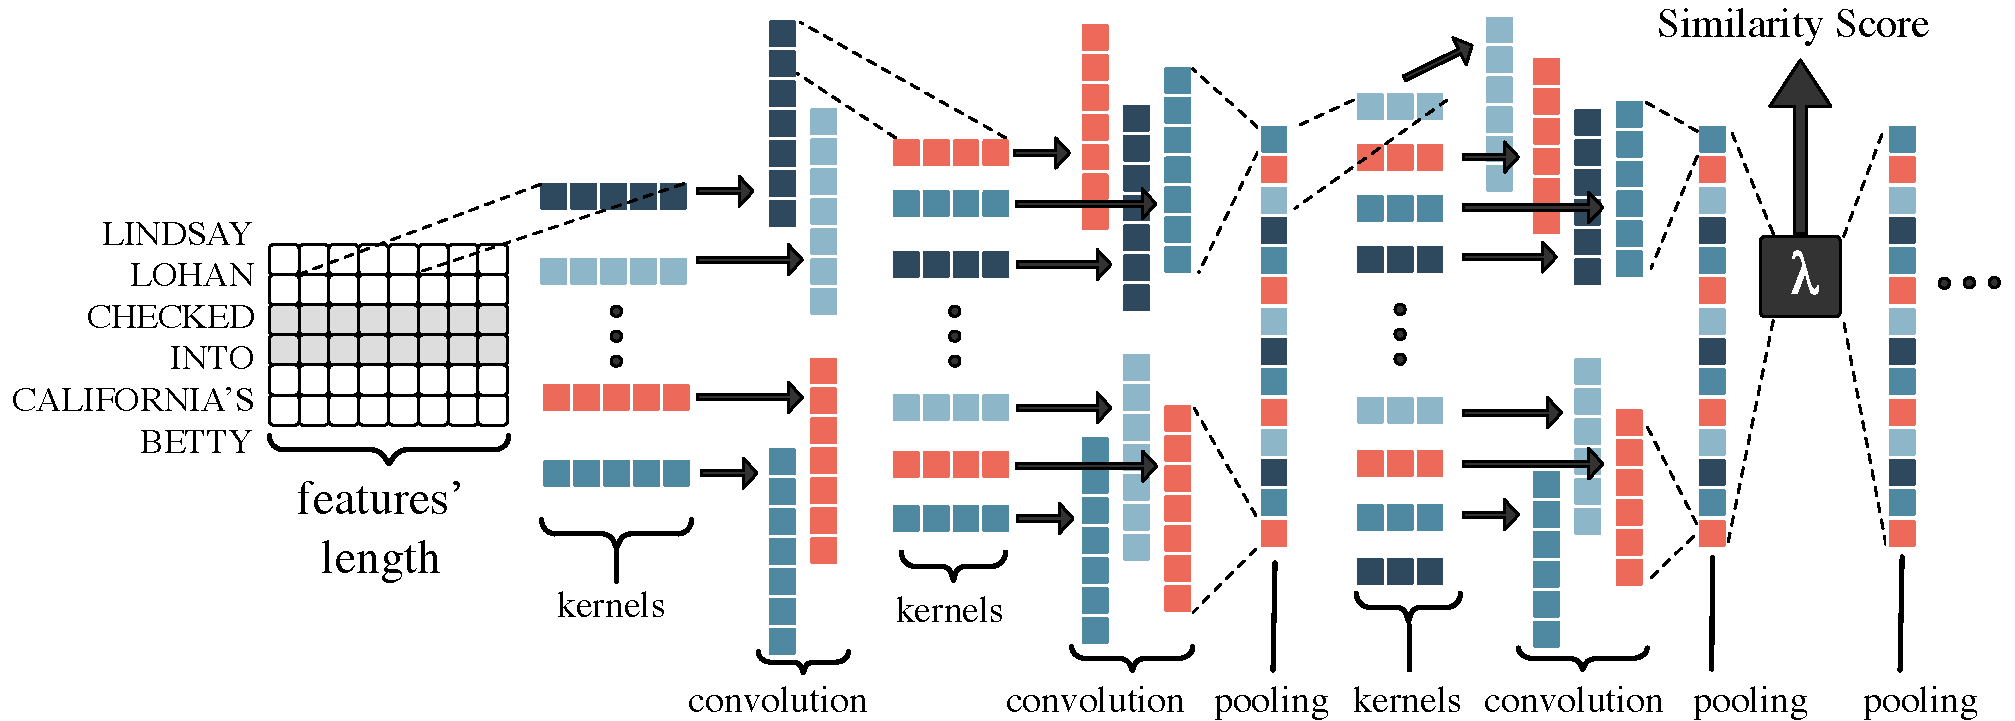
\includegraphics[width=1\textwidth]{architecture.pdf}
	\caption{One half of the Conjoined Convolutional Neural Network's Architecture.}
	%\caption{Conjoined Convolutional Neural Network's Architecture.  The left half shares the same weights with the right half.  Blocks A, C, and F represent 32, 64, and 128 kernels, respectively.  The kernel size is 1x3, and different colors denote distinct kernels.  Blocks B, D, and G represent Convolution with stride of 1, ReLU activation, then 10\% dropout.  Blocks E and H represent MaxPooling with kernel size 1x2.  The Lambda function in the center represents the Euclidean Distance of the merged univariate vectors.}
	\label{fig:ccnn}
\end{figure*}

\subsection{Loss / Optimization}
Our goal is to maximize discriminability of different event mentions, while enforcing features to be as similar as possible when they are of the same event.  Contrastive Loss, shown in Equation \ref{eq:contrastive}, is perfectly suited for this objective \cite{SchroffKP15,pmlr-v48-liud16}. Our training set has a strong class imbalance (most input pairs are not co-referent), so we down-sample to a 5:1 ratio of negative-to-positive examples.  We use Adagrad for optimization.
\begin{equation}
\begin{aligned}
L(&\hat{y},y)=\frac{1}{2N}\sum_{n=1}^{N}[(y)d^2 \\
&\qquad {} + (1-y)*(max(1-d,0))^2] \\
&\textnormal{where }d=\|y_{n}-\hat{y}_{n}\|_{2}
\end{aligned}
\label{eq:contrastive}
\end{equation}

%%%%%%%%%%%%%%%%%%%%%%%%%%%%%%%%%%%%%%%%%%%%%%%%%
%%%%%%%%%%%%%                5.   NEURAL CLUSTERING                %%%%%%%%%%%%%%%
%%%%%%%%%%%%%%%%%%%%%%%%%%%%%%%%%%%%%%%%%%%%%%%%%

\section{Neural Clustering (NC)}
\label{sec:clustering}
It is common practice for mention-pair models to first assign a probability score to every mention-pair, and then cluster with a different model.

\subsection{Existing Clustering Approaches}
\textbf{Agglomerative Clustering} is a simple but effective approach.  It first assigns each mention to its own singleton cluster.  Then, it repeatedly merges the two distinct clusters which contain the shortest-distance mention pairs.  Although this is a strong baseline, as seen in Yang, et. al. \shortcite{journals/tacl/YangCF15}, there are three main weaknesses:
\begin{enumerate}
\item One must define a stopping threshold $\alpha$.
\item Any given $\alpha$ hinges on the data being uniform across documents.  In reality, distances between mention-pairs could vary significantly between documents and topics.
\item Most significant, each cluster merge is based solely on two individual mentions, yet these mentions may not be representative of the cluster at large.
\end{enumerate}

\textbf{HDDCRP and Iterative-Folding Clustering} both contain the issue \#3 from above, as detailed in Sections \ref{sec:HDDCRP} and \ref{sec:Choubey}.

\subsection{Our Approach}
We aim to use the strengths of agglomerative clustering, while replacing its shortcomings.  We train a classifier to learn the most likely {positive cluster merge}, where the cluster is represented more holistically than a mention-pair basis.

Specifically, we learn a function $f(C_x,C_y)$ that predicts the likelihood of an appropriate, positive merging of clusters $(C_x,C_y)$. Let $d(m_i,m_j)$ be the mention-pair distance predicted by our CCNN model, where $m_i \in C_x$, and $m_j \in C_y$.  Function $f(C_x,C_y)$ is based on four simple features:
\begin{itemize}
  \item min-pair distance: $\min_{m_i,m_j} d(m_i,m_j)$
  \item avg-pair distance: $\frac{\sum_{m_i, m_j} d(m_i,m_j)}{\|C_x\|\|C_y\|}$
  \item max-pair distance: $\max_{m_i,m_j} d(m_i,m_j)$
  \item size of candidate cluster: $\frac{\|C_x\| + \|C_y\|}{\sum_{z}{\|C_z\|}}$
\end{itemize}

The first three features serve to better represent the cluster at large (issue \#3 from above).  For example, a given cluster $C_1$, when evaluated against two other candidate clusters $C_2$ and $C_3$, may have the same minimum mention-pair distance score with both $C_2$ and $C_3$  Yet, the average and maximum distance scores shed more light onto which cluster has more similar mentions. Cluster size represents the size percentage of our considered merge, relative to all mentions in our current set.  This may help prevent clusters from growing too large, and is not as vulnerable to issue \#2.

\subsection{Architecture}
We define $f$ as a feed-forward neural network\footnote{We used 1 hidden layer of 25 units, ReLU activation without dropout, and Adagrad as our optimizer.} which predicts the probability of a positive cluster merge, via a two-class softmax function.  Our loss function is weighted binary cross-entropy, to account for the class imbalance situation that most pairs of clusters should not be merged together.  

\subsection{Inference}
Our system will incrementally build up clusters, starting with each cluster having just one mention (in the within-document scenario).  Thus, it is important to train our Neural Clustering model on positive and negative examples of clusters in varying states of completeness.  Our gold truth data informs us which mentions are co-referent, but since there is no single canonical ordering in which mentions should become co-referent, we generate synthetic data to represent possible positive and negative examples of when clusters should be merged.

Specifically, for training, we generate a positive example by randomly sampling a golden cluster, followed by splitting the cluster into two random subsets.  The above four features are calculated for these two subsets of clusters, and the target output is a positive case.  Likewise, we generate negative examples by sampling random subsets from disjoint golden clusters.

At test time, we use Neural Cluster to evaluate every possible $(C_x, C_y)$ cluster pair in an easy-first manner.  That is, at each iteration, we merge only the $(C_x,C_y)$ pair that yielded the highest likelihood of a positive merge.  Then, we re-evaluate all pairs with our newly merged cluster, and repeat until the model no longer predicts merge.  Thus, unlike aforementioned models, we do not \textit{require} additional stopping parameters.

%%%%%%%%%%%%%%%%%%%%%%%%%%%%%%%%%%%%%%%%%%%%%%%%%
%%%%%%%%%%%%%%           6.   COREFERENCE SYSTEMS           %%%%%%%%%%%%%%%
%%%%%%%%%%%%%%%%%%%%%%%%%%%%%%%%%%%%%%%%%%%%%%%%%
\section{Our Coreference Systems}
\label{sec:coreference}

We use our CCNN and Neural Clustering (NC) models together to perform coreference resolution. The only differences between the within-document and cross-document scenarios are our data and evaluation metric, as described below.

\subsection{Training / Development / Testing Data}
We adhere to the same data splits as previous researchers, whereby the dev set is topics 23-25, and the test set is topics 26-45.  Traditionally, topics 1-22 are used as training.  However, since our NC model relies on our CCNN's predictions, we remove topics 19-22 from the training set and instead use them as dev sets for our NC models.  The complete details are provided in our Supplemental Materials document.

\subsection{Within-Document}
We train a CCNN model on mention-pairs which appear in the same document, and using its predictions on a held-out set, we train the NC to predict when to merge clusters.

\subsection{Cross-Document}
Cross-document resolution is a superset of the within-document task; it uses all coreference chains, regardless if mentions in a cluster were originally from the same document or not.  Our cross-document and within-document systems are identical, except: (1) we train a separate CCNN only on mention-pairs which are from different documents; (2) instead of initializing our clustering with all singleton clusters, we use our within-document NC predictions as starting clusters; (3) at each iteration, we only consider merging clusters $(C_x,C_y)$ if $C_x$ and $C_y$ contain mentions from disjoint sets of documents.  Our cross-document NC only uses cross-document mention pairs distances for its decisions.  Thus, cross-document merging will never merge two within-document clusters from the same document.
%%%%%%%%%%%%%%%%%%%%%%%%%%%%%%%%%%%%%%%%%%%%%%%%%
%%%%%%%%%%%%%%                         7.          RESULTS                  %%%%%%%%%%%%%%%
%%%%%%%%%%%%%%%%%%%%%%%%%%%%%%%%%%%%%%%%%%%%%%%%%
\section{Results}
As a recap, our research concerns three independent axis of investigation:
\begin{itemize}
\item \textbf{Features:} which features are most useful, and can we use few features?
\item \textbf{Mention-Pair Model:} how well does CCNN perform against a standard feed-forward neural network\footnote{Given two mentions $i$ and $j$, with corresponding feature vectors $f_i$ and $f_j$, their input to the Feed-Forward Neural Network is the vector $\|f_{i} - f_{j}\|$} (FFNN)?
\item \textbf{Clustering:} can we outperform Agglomerative via our Neural Clustering model?
\end{itemize}

Our metric is CoNLL F1 score, which is a clustering-based metric that combines the F1 scores of MUC, $B^{3}$, and $CEAF_{e}$, and we use the official scorer script (v8.01) \cite{Pradhan+etal:14a}.

\begin{figure*}[h]
\centering
	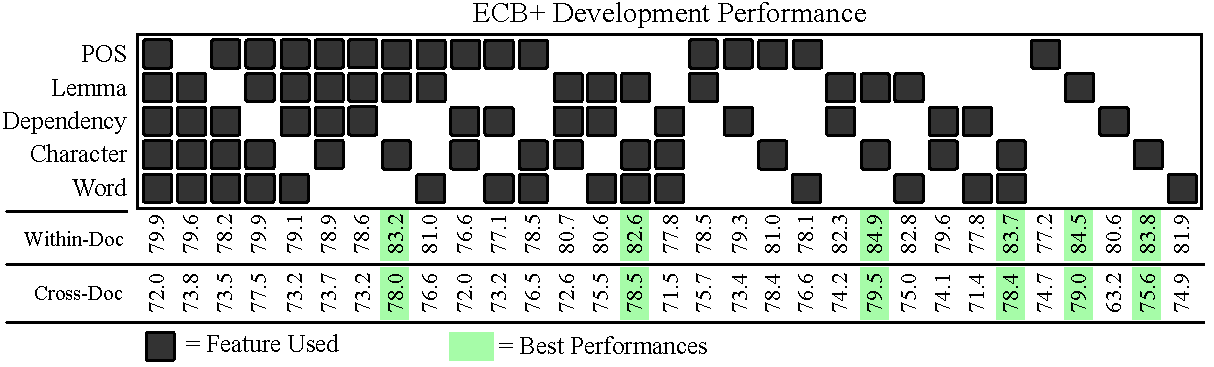
\includegraphics[width=0.82\textwidth]{features.pdf}
	\caption{The CoNLL F1 performance of our flagship CCNN + Neural Clustering system, using all combinations of features.}
	\label{fig:allfeatures}
\end{figure*}

We were interested in the five common, non-relational embedding features which are detailed in Section \ref{sec:features}: POS, Lemma, Dependency Lemma, Character, Word.  We tested all combinations of features on the Dev Set, and Lemma + Character Embedding yielded the best dev results (see Figure \ref{fig:allfeatures}).  Thus, our CCNN + Neural Clustering system used only these two features in its evaluation against other systems (see Table \ref{tab:others}).  The results show that our CCNN model outperforms a FFNN, and that our Neural Clustering outperforms Agglomerative Clustering.  Further, when training and testing on gold mentions, we achieved CoNLL F1 scores of \textbf{81.2} and \textbf{72.4} for within-document and cross-document, respectively.  We denote these scores as the new baseline to which to compare future systems.

\begin{table*}[h]
\centering
\tabcolsep=0.15cm
\begin{tabular}{r|ccc|c|ccc|c|}
\cline{2-9}
& \multicolumn{4}{|c|}{Within-Document} & \multicolumn{4}{|c|}{Cross-Document}\\
\cline{2-9}
& \multicolumn{1}{c}{MUC} & B$^3$ & CEAF & CoNLL F1 & \multicolumn{1}{c}{MUC}& B$^3$ & CEAF & CoNLL F1\\
\hline
 \multicolumn{9}{|c|}{Test Set: ECB+ Gold Mentions} \\
 \hline
 \multicolumn{1}{ |c| }{SameLemma}& 58.3 & 83.0 & 75.9 & 72.4 & 84.2 & 68.2 & 48.0 & 66.8 \\
\multicolumn{1}{ |c| }{FFNN+AGG} & 59.9 & 85.6 & 78.4 & 74.6 & 77.7 & 69.9 & 50.1 & 65.9\\
\multicolumn{1}{ |c| }{FFNN+NC} & 60.7 & 86.7 &  79.4 & 75.6 & 74.9 & 67.8 & 56.3 & 67.0\\
\multicolumn{1}{ |c| }{CCNN+AGG} & 70.5 & 89.1 & 83.5  & 81.0 & 84.1 & 70.7 & 55.5 & 70.1\\
\multicolumn{1}{ |c| }{\textbf{CCNN+NC}}& 70.9 & 88.9 & 83.6 & \textbf{81.2} & 86.4 & 71.7 & 59.1 & \textbf{72.4}\\
\hline
\hline
 \multicolumn{9}{|c|}{Test Set: HDDCRP's Predicted Mentions} \\
 \hline
\multicolumn{1}{ |c| }{SameLemma}& 40.4 & 66.4 & 66.2 & 57.7 & 66.7 & 51.4 & 46.2 & 54.8 \\
\multicolumn{1}{ |c| }{HDDCRP}& 53.4 & 75.4 & 71.7  & 66.8 & 73.1 & 53.5 & 49.5 & 58.7\\
\multicolumn{1}{ |c| }{\textbf{CCNN+NC}} & 54.0 & 75.5 & 72.2  & \textbf{67.2} & 71.3 & 57.0 & 49.6 & \textbf{59.3}\\
 \hline
\hline
 \multicolumn{9}{|c|}{Test Set: Choubey's et. al. Mentions} \\
 \hline
\multicolumn{1}{ |c| }{SameLemma}& 48.8 & 66.7 & 65.1 & 60.2 &  68.1 & 53.3 & 47.2 & 56.2\\
\multicolumn{1}{ |c| }{Choubey}& 62.6 & 72.4 & 71.8  & 68.9 & 73.4 & 80.4 & 56.5 & 63.6\\
\multicolumn{1}{ |c| }{\textbf{CCNN+NC}} & 67.3 & 73.0 & 69.5  & \textbf{69.9}& 77.0 & 56.3 & 60.2 & \textbf{64.5}\\
 \hline
\end{tabular}
\caption{Comparison against other systems, while our models use only the Lemma + Character Embedding features.  FFNN denotes a Feed-Forward Neural Network Mention-Pair model.  AGG denotes Agglomerative Clustering.}
\label{tab:others}
\end{table*}

\textbf{Lemma Embeddings} were the most useful feature, followed closely by Character Embeddings.  Since \textit{SameLemma} has historically been a strong baseline, this is unsurprising.  

\textbf{Character Embeddings} were effective for the same reason String Edit Distance is often a strong feature: there tends to be a direct correlation between the textual similarity of mentions and their likelihood of being co-referent. Both random character embeddings and pre-trained ones yielded the same performance, suggesting that the power comes from the uniqueness of characters, not any \textit{meaning} conveyed in the characters.

Empirically, Lemma + Character Embeddings are complementary features; the semantic information conveyed within the lemma embeddings complement the syntactic information of character embeddings.  Related, POS by itself was a poor feature, but combining it with either Lemma or Character Embeddings offered strong results. 

Ideally, a classifier should learn how to combine all features such that the unhelpful ones are given no weight.  However, in practice, that is often extremely difficult, due to both the large parameter space and high entropy wherein some combinations of features seem to equally help as much as hurt.  Thus, we conclude that one should try to use the fewest features as possible for coreference resolution, then expand appropriately.

%Interestingly, in all experiments, our results were inversely correlated with the amount of context our CCNN used.  That is, our best performance came when we used no context, only the mention words.  This agrees with the Choubey's, et. al. findings \shortcite{Choubey2017EventCR}.

\subsection{Comparison to Other Systems}
\textit{SameLemma} has historically proven to be a strong baseline.  That is, anytime two mentions have identical lemmas, simply mark them as being co-referent.

Using the same mentions that were used by the HDDCRP and Choubey (Iteratively-Unfolding) systems, our flagship CCNN+NC system yielded the highest results, despite using few features.


\subsection{Error Analysis}
\textbf{False Positives} include mentions which are textually identical but not actually co-referent (e.g., \textit{placed} and \textit{placed}, which only differ in their direct objects).  \textbf{False Negatives} include abbreviations (e.g., \textit{i.r.} and \textit{injured reserve}) and colloquial phrases (e.g., The \textbf{casting} of Smith; (2) Smith \textbf{stepped into} the role; (3) was \textbf{handed the keys}).

Since our cross-document system relies on the within-document predictions, it is easy for errors to propagate.

%(1) The Saints \textbf{placed} rookie Chris Ivory on injured reserve Tuesday [...] and (2) The saints have \textbf{placed} running back Pierre Thomas on injured reserve.  These sentences have different direct objects, so the ECB+ corpus denotes them as being non-coreferent.


%%%%%%%%%%%%%%%%%%%%%%%%%%%%%%%%%%%%%%%%%%%%%%%%%
%%%%%%%%%%%%%%                     8.         CONCLUSION               %%%%%%%%%%%%%%%
%%%%%%%%%%%%%%%%%%%%%%%%%%%%%%%%%%%%%%%%%%%%%%%%%

\section{Conclusion}
In summary, we present a novel approach to event coreference resolution that uses a Conjoined Convolutional Neural Network as a mention-pair model, followed by a Neural Clustering model.  Unlike most coreference systems which rely on dozens of features, we used only lemmatization and pre-trained word/character embeddings.  We illustrate the performance of five commonly used features, demonstrating the effectiveness of using few features.  Our Neural Clustering model addressed a common weakness in mention-pair models: instead of forming clusters based on just \textit{one} mention-pair satisfying a criterion, we used features which represent clusters more holistically.  On a common test set, our system achieved state-of-the-art performance with CoNLL F1 scores of 67.2 and 59.3 for within-document and cross-document, respectively.  Further, using gold mentions, we set a new within-document baseline of 81.2 and cross-document baseline of 72.4.

% include your own bib file like this:
%\bibliographystyle{acl}
%\bibliography{acl2018}
\bibliography{acl2018}
\bibliographystyle{acl_natbib}

\appendix


\end{document}
